\section{Discussion of Results}
\label{sec:discussionofresults}

\subsection{Influence of some parameters in our model}

\subsubsection{Influence of \texttt{maxAgentupdate}}
\label{sec:maxAgentUpdate}
As the figure \ref{influencemaxAgentUpdate} shows the value for \texttt{maxAgentupdate} just gives us a different scaling of the time axis. If it is bigger the total residual rises faster while if it is smaller the total residual rises slower. As a result of this a change in the value of \texttt{maxAgentupdate} could help to speed up the simulation in order to get quicker results.

\begin{figure}
\centering
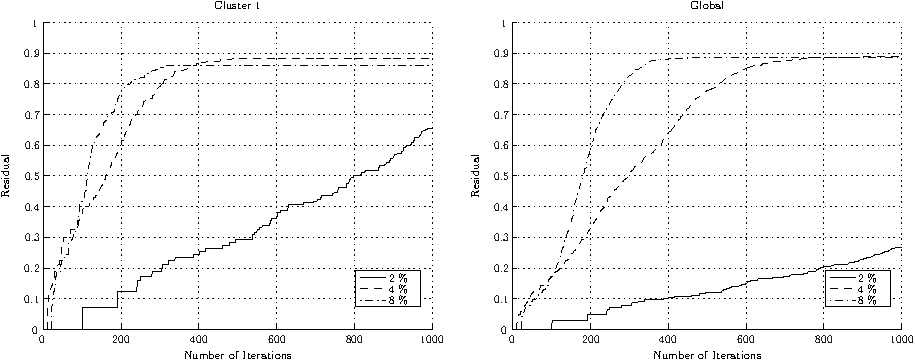
\includegraphics[width= \textwidth]{influenceOfmaxUpdate/influenceMaxAgentUpdate.pdf}
\caption{On the left the residual for the cluster in which the riots started is plotted while on the right the global residual is shown. In both it is shown for values of 0.02, 0.04 and 0.08 of \texttt{maxAgentupdate}}
\label{influencemaxAgentUpdate}
\end{figure}


\subsubsection{Influence of \texttt{noize}}
\label{sec:influencenoize}
As figure \ref{influencenoize} shows, the noize could have quite an influence on the results of the simulation. In our network we have in total 1200 nodes. All the simulations in figure \ref{influencenoize} have the same \texttt{maxUpdate}=0.02. This means that in every time step 24 agents get updated. If the noize is now for example 0.01 only 0.24 agents choose randomly their state. In the case of a noize of 0.1 get 2.4 agents every time step a randomly after a uniform distribution chosen mind state. After this "noize update" the concerned agents are removed from the sequential update list so that they could not be updated twice.\\
As figure \ref{influencenoize} now shows and explained above a noize of 0.01 does not really change the results of the simulation as it has nearly no influence. But as the series of five plots on the right in figure \ref{influencenoize} shows a noize of 10 $\%$ does have quite a big influence on the results of the simulation. Before this big noize the riots where not really starting in the networks now they spread quickly.\\
Compared to reality we think that the noize tends to be close to 0. Who is just completly random changing his mind? It could be that some people change their mind independently from their neighbors and these should be covered by the noize. We think that a noize in reality should be something between 0 and 0.06.

\begin{figure}
\centering
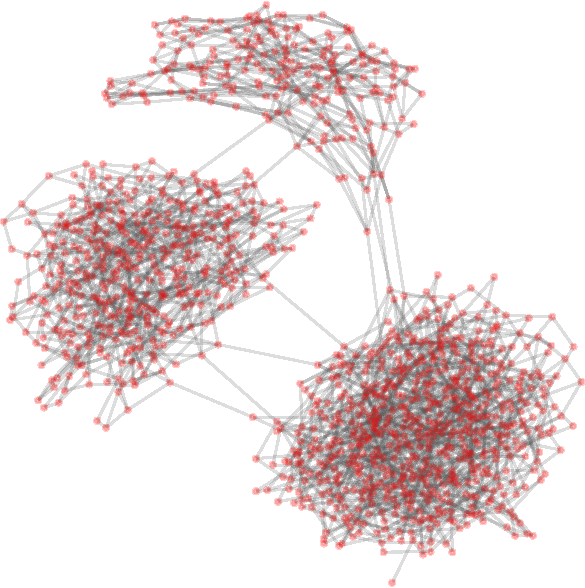
\includegraphics[width=0.25\textwidth]{batchRun__kHalf=2-2-2_maxUpdate=0.02_noize=0_nbrDepth=1/network0-crop.pdf}
\hfill
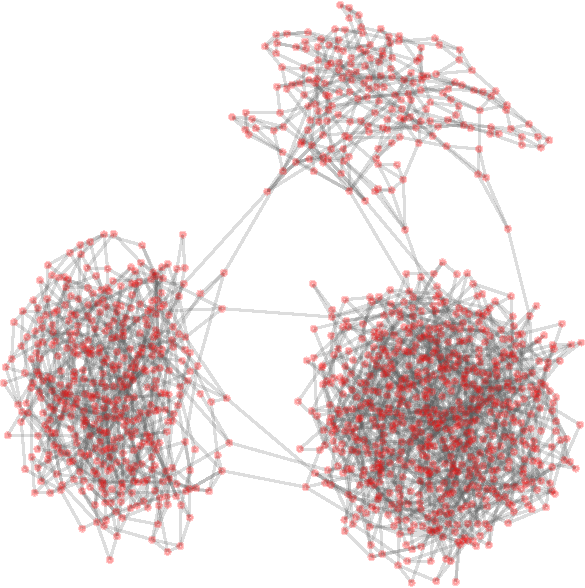
\includegraphics[width=0.25\textwidth]{batchRun__kHalf=2-2-2_maxUpdate=0.02_noize=0.01_nbrDepth=1/network0-crop.pdf}
\hfill
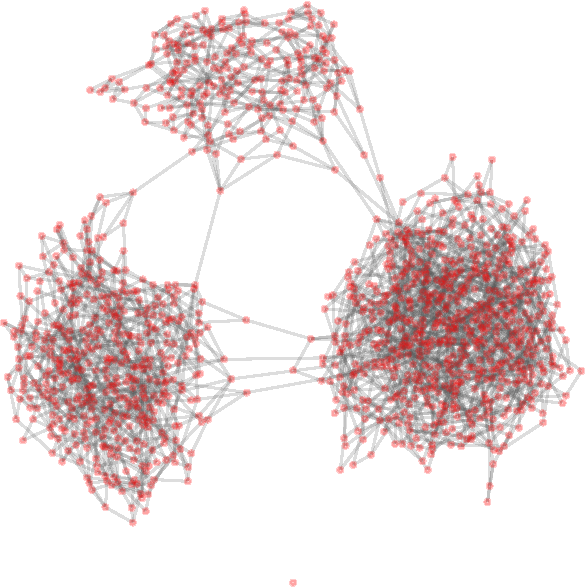
\includegraphics[width=0.25\textwidth]{batchRun__kHalf=2-2-2_maxUpdate=0.02_noize=0.1_nbrDepth=1/network0-crop.pdf}

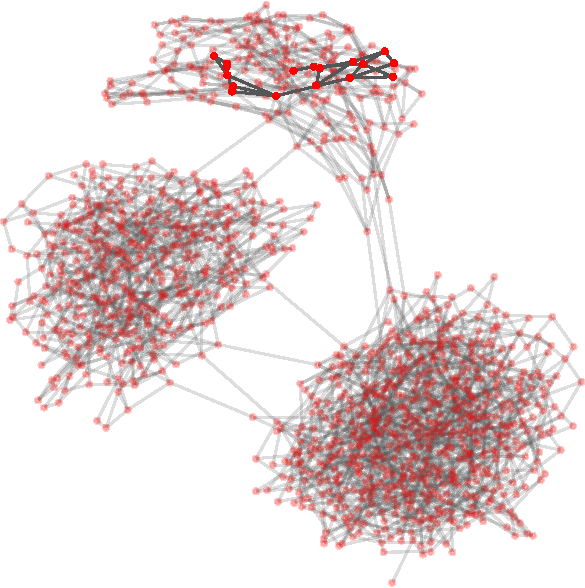
\includegraphics[width=0.25\textwidth]{batchRun__kHalf=2-2-2_maxUpdate=0.02_noize=0_nbrDepth=1/network250-crop.pdf}
\hfill
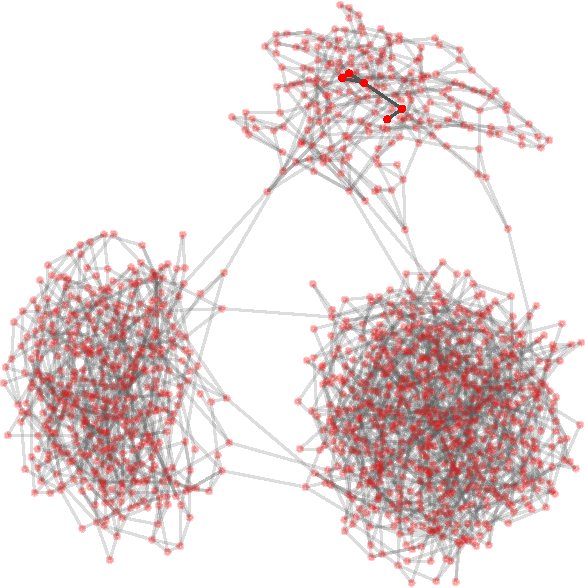
\includegraphics[width=0.25\textwidth]{batchRun__kHalf=2-2-2_maxUpdate=0.02_noize=0.01_nbrDepth=1/network250-crop.pdf}
\hfill
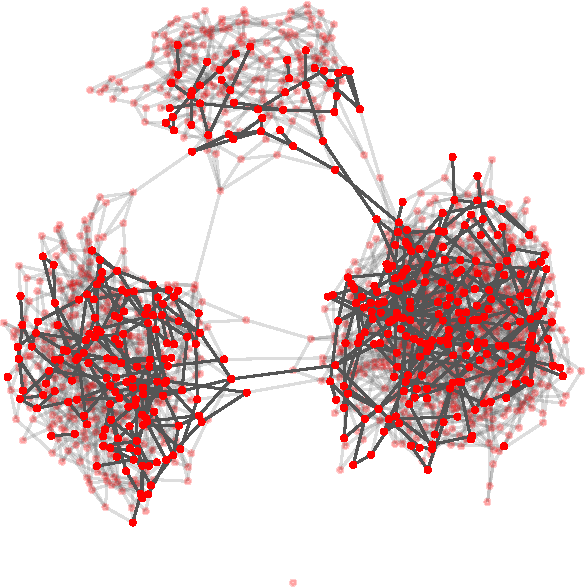
\includegraphics[width=0.25\textwidth]{batchRun__kHalf=2-2-2_maxUpdate=0.02_noize=0.1_nbrDepth=1/network250-crop.pdf}

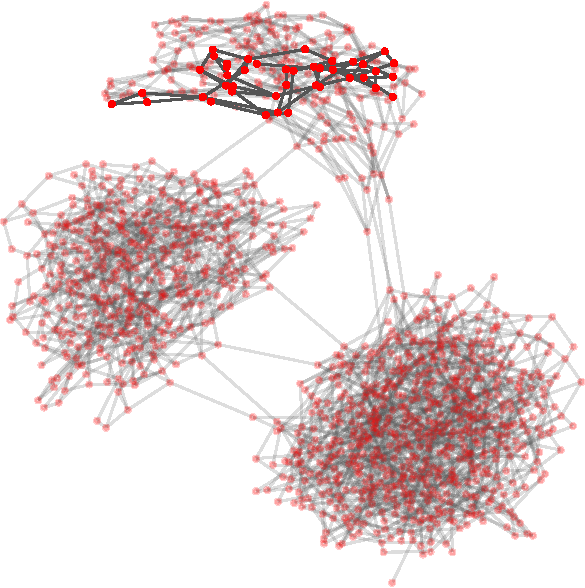
\includegraphics[width=0.25\textwidth]{batchRun__kHalf=2-2-2_maxUpdate=0.02_noize=0_nbrDepth=1/network500-crop.pdf}
\hfill
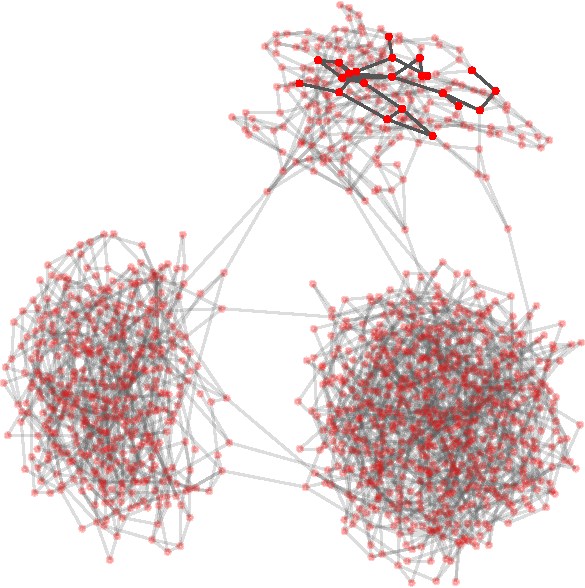
\includegraphics[width=0.25\textwidth]{batchRun__kHalf=2-2-2_maxUpdate=0.02_noize=0.01_nbrDepth=1/network500-crop.pdf}
\hfill
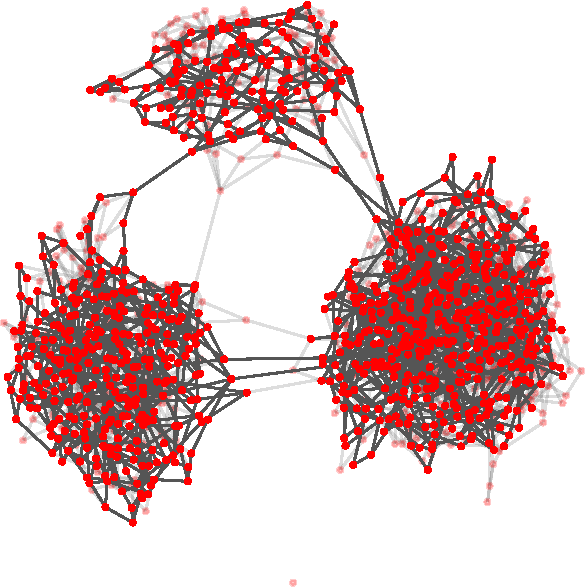
\includegraphics[width=0.25\textwidth]{batchRun__kHalf=2-2-2_maxUpdate=0.02_noize=0.1_nbrDepth=1/network500-crop.pdf}


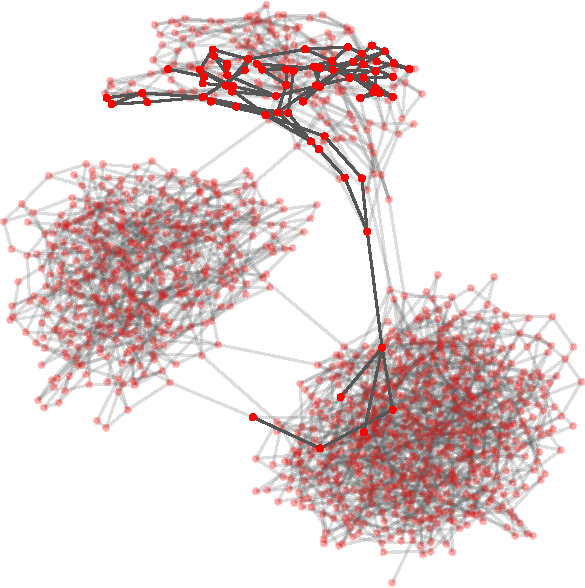
\includegraphics[width=0.25\textwidth]{batchRun__kHalf=2-2-2_maxUpdate=0.02_noize=0_nbrDepth=1/network750-crop.pdf}
\hfill
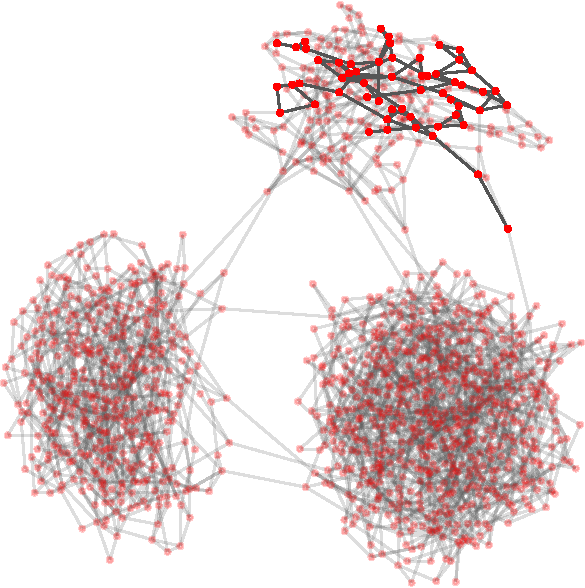
\includegraphics[width=0.25\textwidth]{batchRun__kHalf=2-2-2_maxUpdate=0.02_noize=0.01_nbrDepth=1/network750-crop.pdf}
\hfill
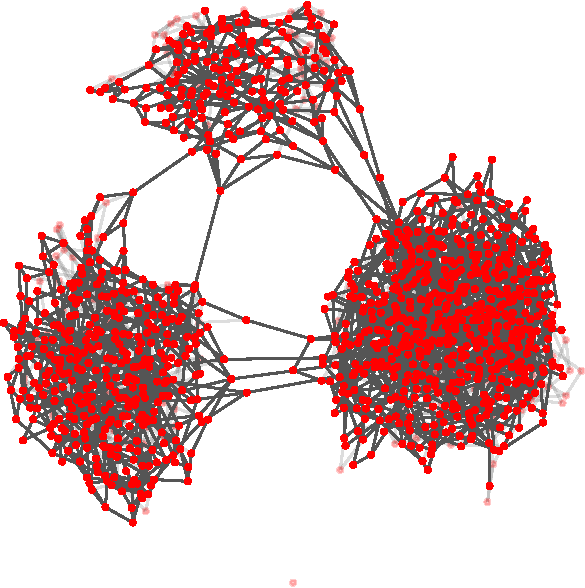
\includegraphics[width=0.25\textwidth]{batchRun__kHalf=2-2-2_maxUpdate=0.02_noize=0.1_nbrDepth=1/network750-crop.pdf}

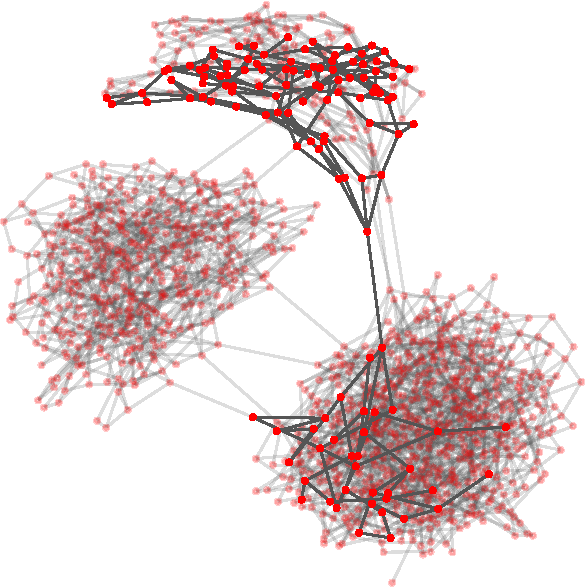
\includegraphics[width=0.25\textwidth]{batchRun__kHalf=2-2-2_maxUpdate=0.02_noize=0_nbrDepth=1/network1000-crop.pdf}
\hfill
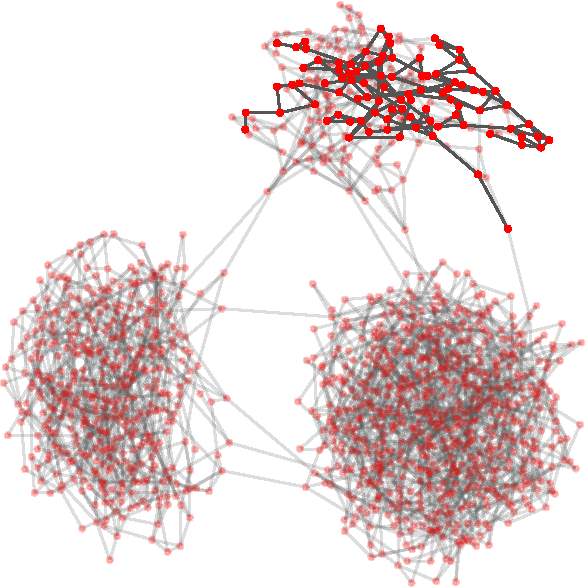
\includegraphics[width=0.25\textwidth]{batchRun__kHalf=2-2-2_maxUpdate=0.02_noize=0.01_nbrDepth=1/network1000-crop.pdf}
\hfill
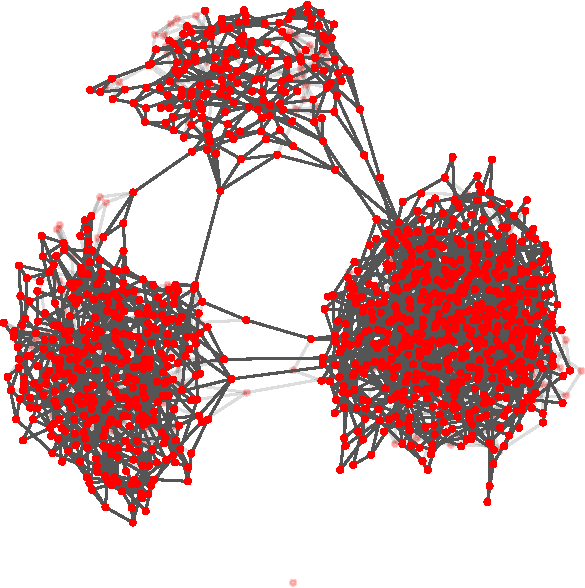
\includegraphics[width=0.25\textwidth]{batchRun__kHalf=2-2-2_maxUpdate=0.02_noize=0.1_nbrDepth=1/network1000-crop.pdf}

\caption{The influence of the noize for the three cases with on the left noize = 0, in the middle 0.01 and on the right 0.1. From top to bottom are the different time steps with the beginning and then increasing in 250 time steps till a 100 time steps.}
\label{influencenoize}
\end{figure}



\subsubsection{Influence of \texttt{nbrDepth} = Neighbor Depth}
\label{sec:nbrDepth}

\begin{figure}
\centering
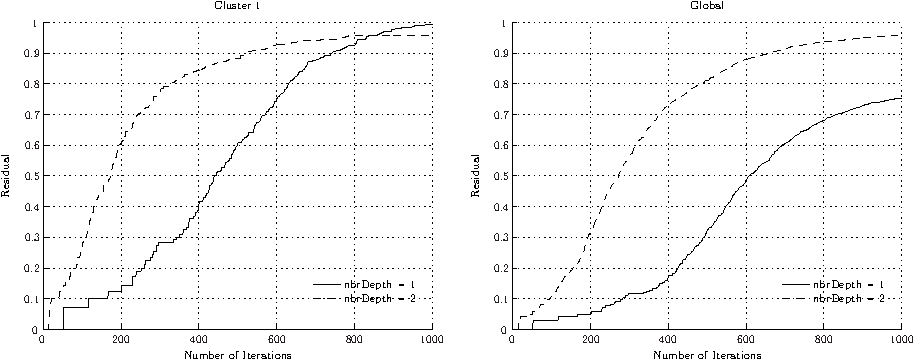
\includegraphics[width= \textwidth]{influenceOfNbrDepth/influenceNbrDepth.pdf}
\caption{The residuals plotted for just cluster 1 on the left and the global residual on the right for neighbor depth 1 and 2. All the other parameters are as in figure \ref{influencenbrdepth}.}
\label{residualNBRdepth}
\end{figure}

As the figure \ref{influencenbrdepth} shows has an iteration over neighbor depth 2 a faster dynamic compared to a neighbor depth of 1. Through a neighbor depth of 2 there is also a quicker jump over from one cluster to the next cluster. This could be explained simpel because there is a high probability that with one node in between there is a link between two clusters. The to this plot belonging residuals are shown in figure \ref{residualNBRdepth}.

\begin{figure}
\centering
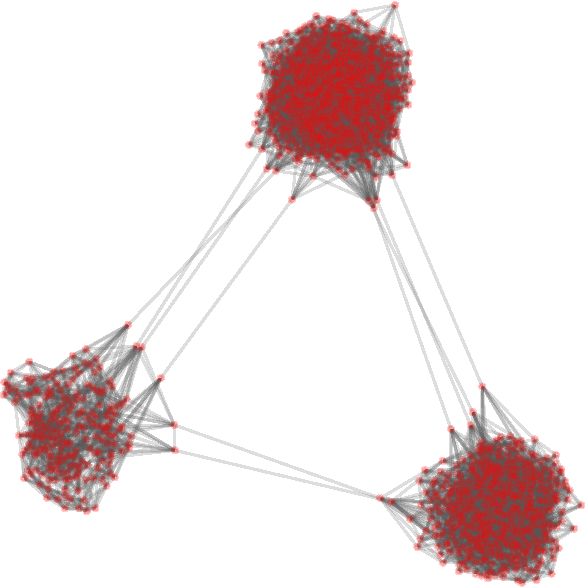
\includegraphics[width=0.3\textwidth]{batchRun__kHalf=6-6-6_maxUpdate=0.02_noize=0_nbrDepth=1/network0-crop.pdf}
\hskip2cm
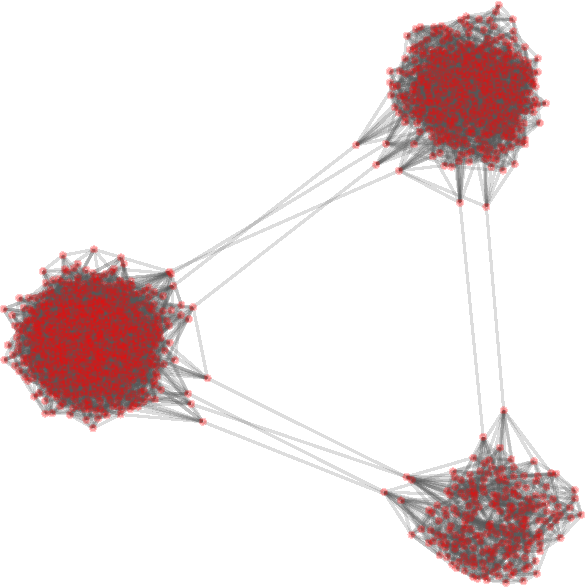
\includegraphics[width=0.3\textwidth]{batchRun__kHalf=6-6-6_maxUpdate=0.02_noize=0_nbrDepth=2/network0-crop.pdf}

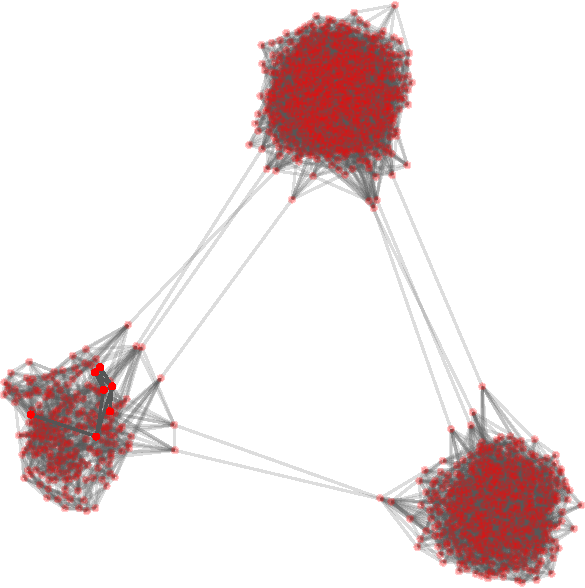
\includegraphics[width=0.3\textwidth]{batchRun__kHalf=6-6-6_maxUpdate=0.02_noize=0_nbrDepth=1/network250-crop.pdf}
\hskip2cm
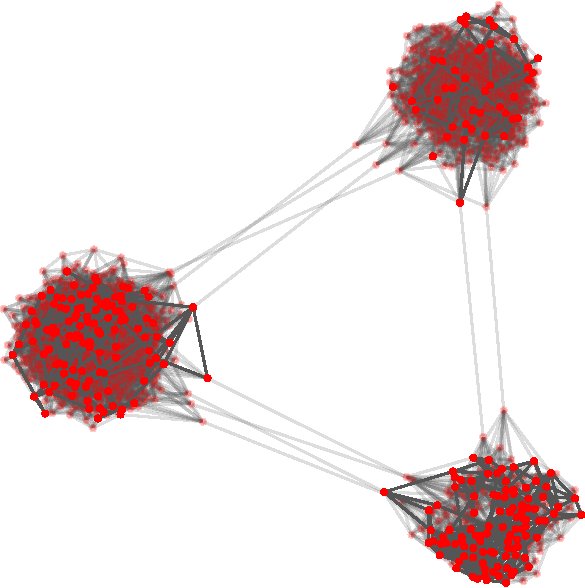
\includegraphics[width=0.3\textwidth]{batchRun__kHalf=6-6-6_maxUpdate=0.02_noize=0_nbrDepth=2/network250-crop.pdf}

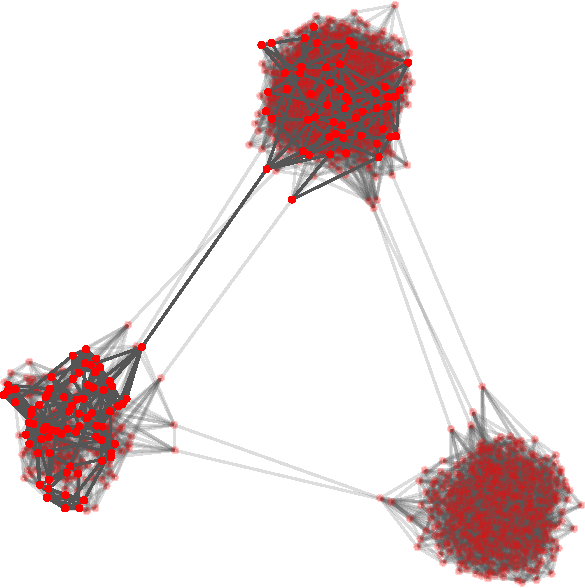
\includegraphics[width=0.3\textwidth]{batchRun__kHalf=6-6-6_maxUpdate=0.02_noize=0_nbrDepth=1/network500-crop.pdf}
\hskip2cm
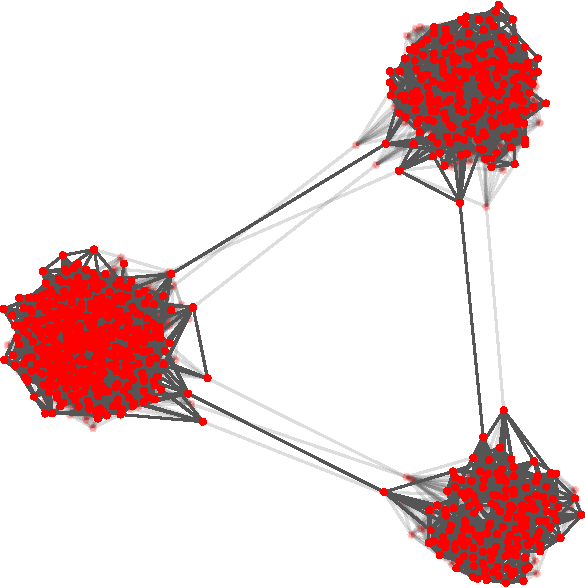
\includegraphics[width=0.3\textwidth]{batchRun__kHalf=6-6-6_maxUpdate=0.02_noize=0_nbrDepth=2/network500-crop.pdf}

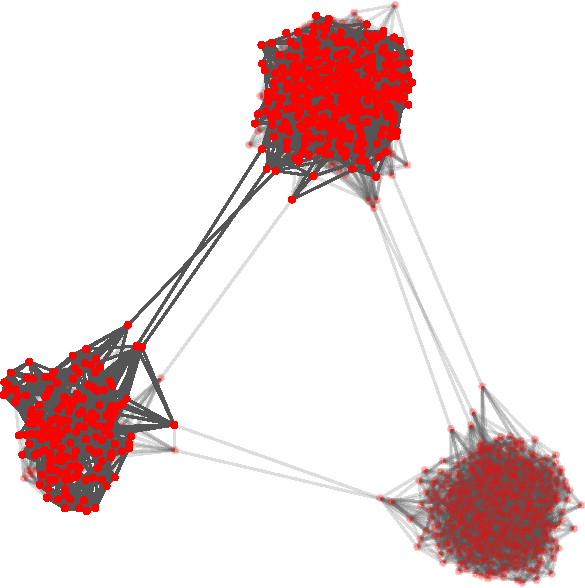
\includegraphics[width=0.3\textwidth]{batchRun__kHalf=6-6-6_maxUpdate=0.02_noize=0_nbrDepth=1/network750-crop.pdf}
\hskip2cm
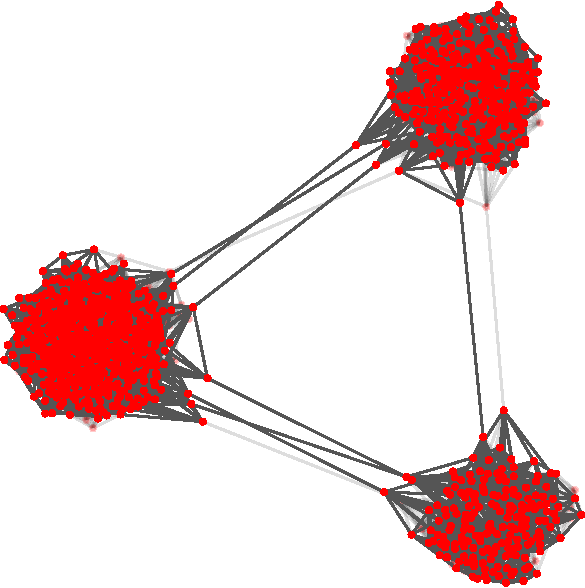
\includegraphics[width=0.3\textwidth]{batchRun__kHalf=6-6-6_maxUpdate=0.02_noize=0_nbrDepth=2/network750-crop.pdf}

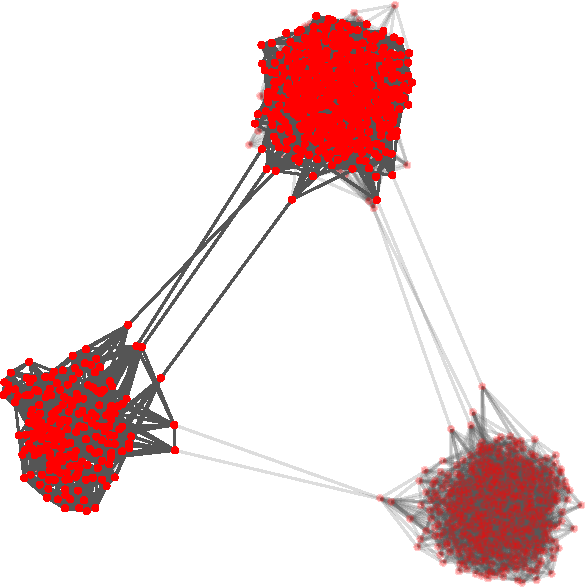
\includegraphics[width=0.3\textwidth]{batchRun__kHalf=6-6-6_maxUpdate=0.02_noize=0_nbrDepth=1/network1000-crop.pdf}
\hskip2cm
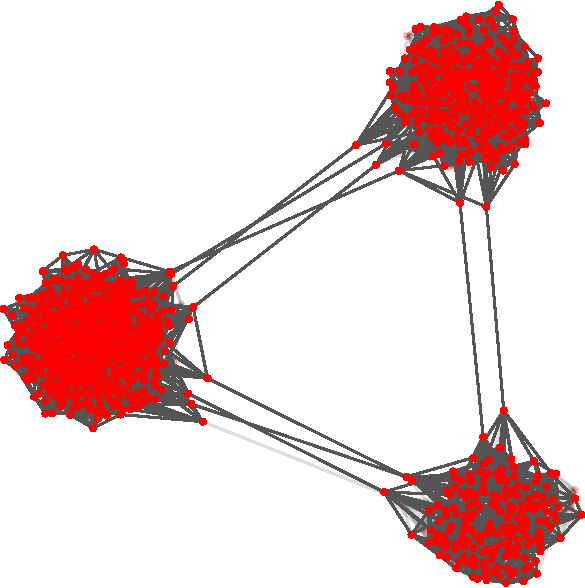
\includegraphics[width=0.3\textwidth]{batchRun__kHalf=6-6-6_maxUpdate=0.02_noize=0_nbrDepth=2/network1000-crop.pdf}

\caption{For this graphs we used a small world network with mean degree 12, a maximal update of 0.02 and 0 noize. In the left series of plots we had a neighbor depth of 1 and in the right series a neighbor depth of 2.}
\label{influencenbrdepth}
\end{figure}

\subsubsection{Influence of the network type}
\label{sec:influencenetworktype}


\begin{figure}
\centering
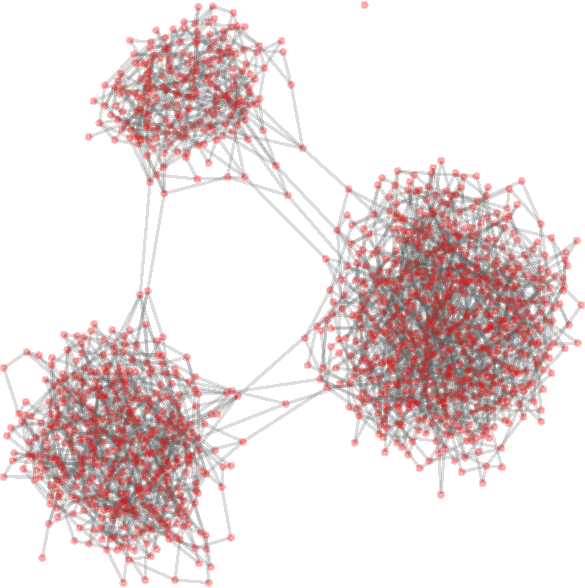
\includegraphics[width=0.3\textwidth]{randomgraphnbrdepth1/network0-crop.pdf}
\hskip2cm
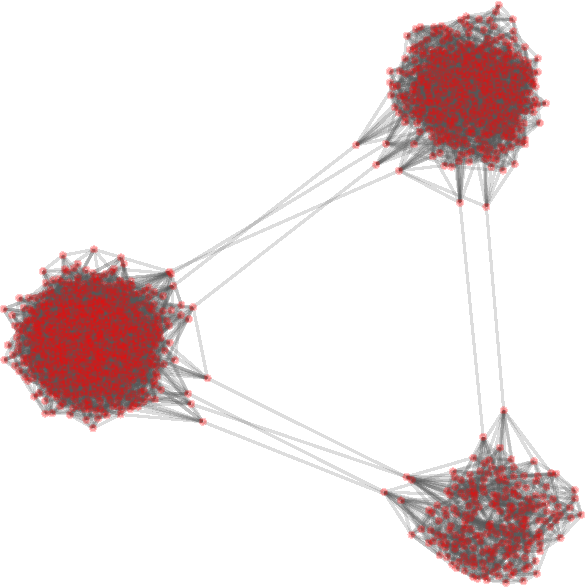
\includegraphics[width=0.3\textwidth]{batchRun__kHalf=6-6-6_maxUpdate=0.02_noize=0_nbrDepth=2/network0-crop.pdf}

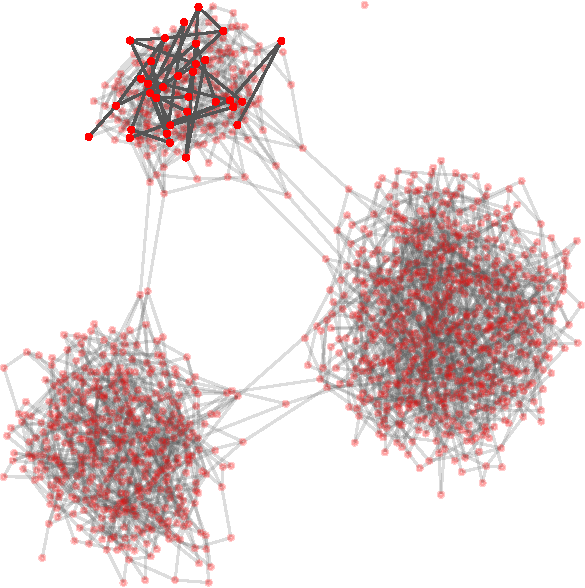
\includegraphics[width=0.3\textwidth]{randomgraphnbrdepth1/network250-crop.pdf}
\hskip2cm
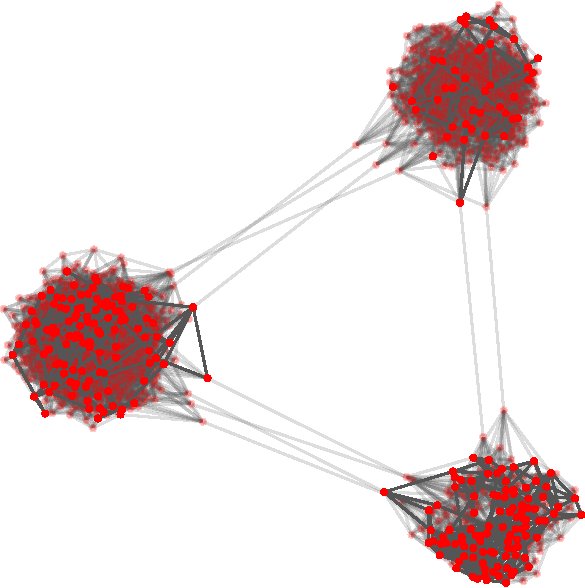
\includegraphics[width=0.3\textwidth]{batchRun__kHalf=6-6-6_maxUpdate=0.02_noize=0_nbrDepth=2/network250-crop.pdf}

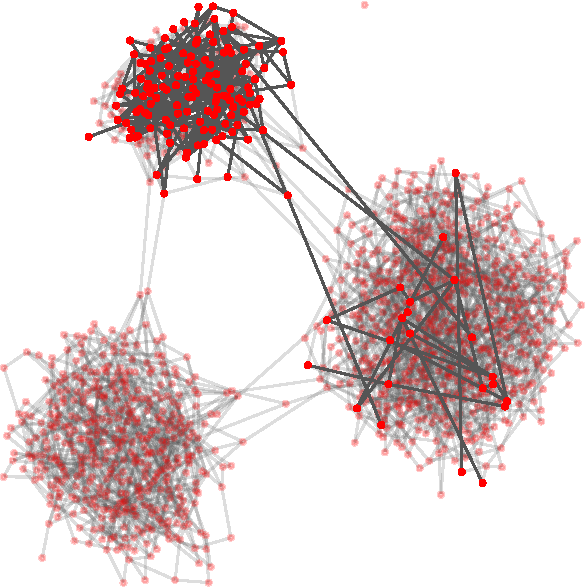
\includegraphics[width=0.3\textwidth]{randomgraphnbrdepth1/network500-crop.pdf}
\hskip2cm
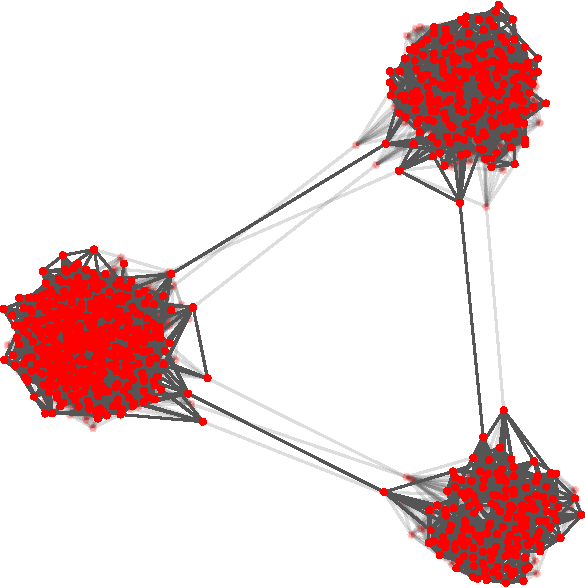
\includegraphics[width=0.3\textwidth]{batchRun__kHalf=6-6-6_maxUpdate=0.02_noize=0_nbrDepth=2/network500-crop.pdf}

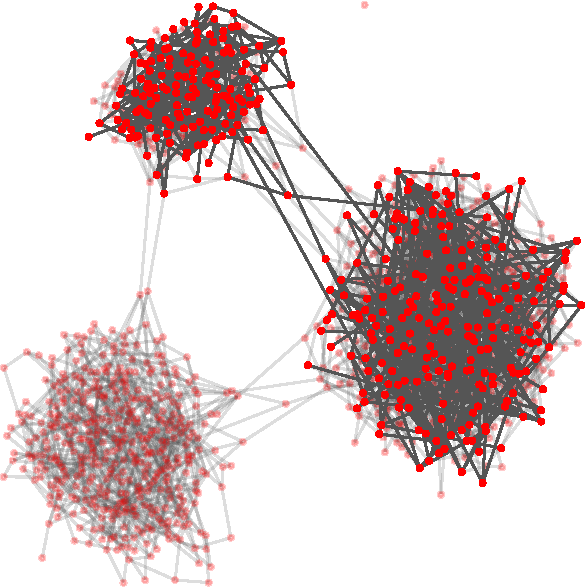
\includegraphics[width=0.3\textwidth]{randomgraphnbrdepth1/network750-crop.pdf}
\hskip2cm
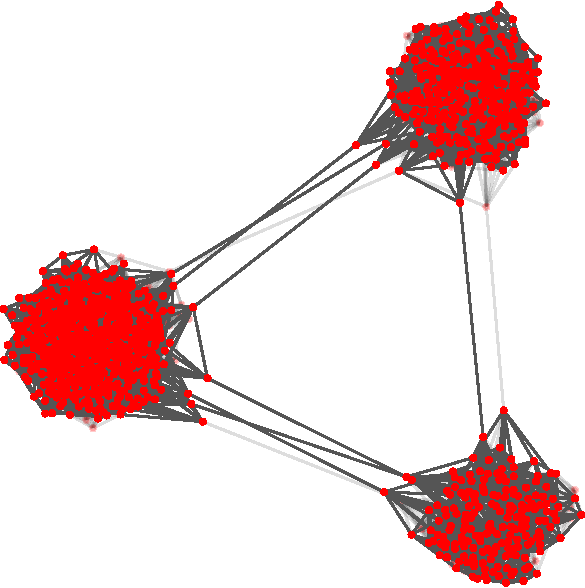
\includegraphics[width=0.3\textwidth]{batchRun__kHalf=6-6-6_maxUpdate=0.02_noize=0_nbrDepth=2/network750-crop.pdf}

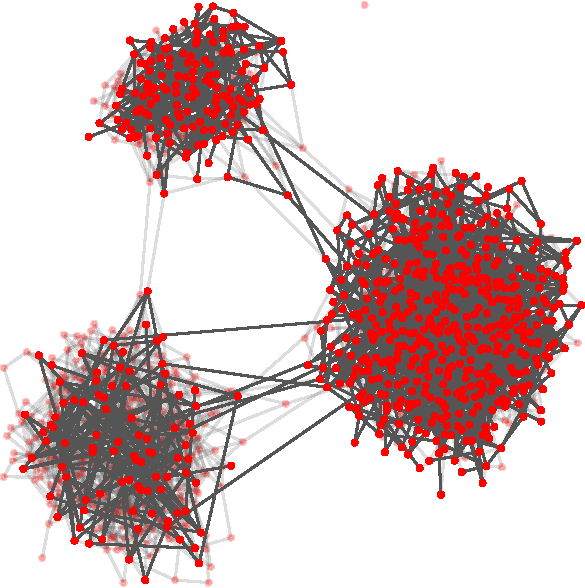
\includegraphics[width=0.3\textwidth]{randomgraphnbrdepth1/network1000-crop.pdf}
\hskip2cm
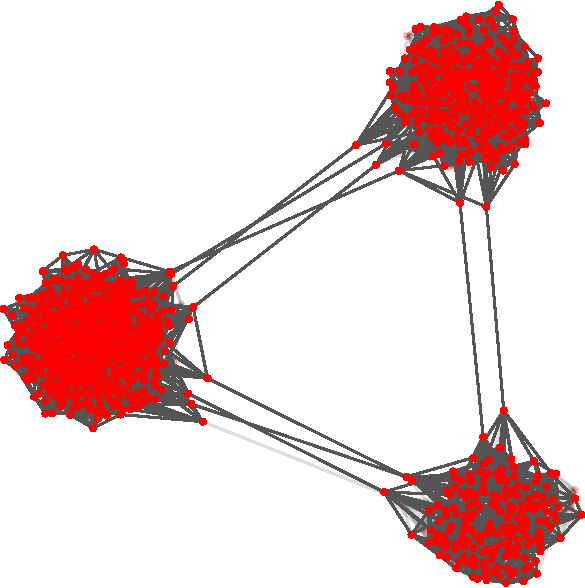
\includegraphics[width=0.3\textwidth]{batchRun__kHalf=6-6-6_maxUpdate=0.02_noize=0_nbrDepth=2/network1000-crop.pdf}

\caption{bla}
\label{influenceNBRdepthRANDOM}
\end{figure}

\subsection{Comparison to reality}
\label{sec:comparisontoreal}